\section{Brake Test}\label{sec:brake-test}

	\subsection{Full Stop Test}\label{ssec:full-stop-test}

		The desired test will be the full stop test, described by \cite{caixeta2017} as a test where the speed is set to a upper limit and then to nought rotation at the end. In order to evaluate the reliability from developed hardware.the test shall be carried a hundred times.

		\par
		In order to start the brake test the following parameters were configured on the \textit{Labview} Test Application as Table \ref{table:brake-test-parameters} shows.

		\begin{table}[h!]
			\begin{tabular}{|l|l|l|}
				\hline
				\textbf{Parameter} & \textbf{Value} & \textbf{Description} \\ \hline
				Number of Snubs & 100 & To achieve reliable data. \\ \hline
				Interval Between Snubs & 5s & Allows the brakes to cool down after each Snub. \\ \hline
				Upper Limit & 500 rpm & Almost the maximum rotation of the rotor (580rpm) \\ \hline
				Upper Wait Interval & 3s & Just enough so that the speed can stabilize \\ \hline
				Lower Limit & 0 rpm & The ideia is to fully stop the system. \\ \hline
				Lower Wait Interval & 1s & Just enough to guarantee no momentum is present. \\ \hline
			\end{tabular}
			\caption{Test Parameters Setup}
			\label{table:brake-test-parameters}
		\end{table}

		The goal of this tests is not to evaluate braking performance of components of a brake system but rather to achieves that the developed hardware can be used for that, i.e. showing that the measured quantities are directly related to the tests are being carried out. Hence, it is expected that temperature should increase after each snub. Morover, as the measured braking pressure increases and the CKP signal frequency should decrease rapidly. Moreover, it shall be possible to see a variation in brake efficiency when the brakes starts to get hotter.

	\subsection{Results and Discussion}\label{ssec:full-stop-test-results}

		Figure \ref{fig:test-first-ten-snubs} shows a graph with the measured quantities on the first ten of the hundred snubs.

		\begin{figure}[htbp]
				\centering
				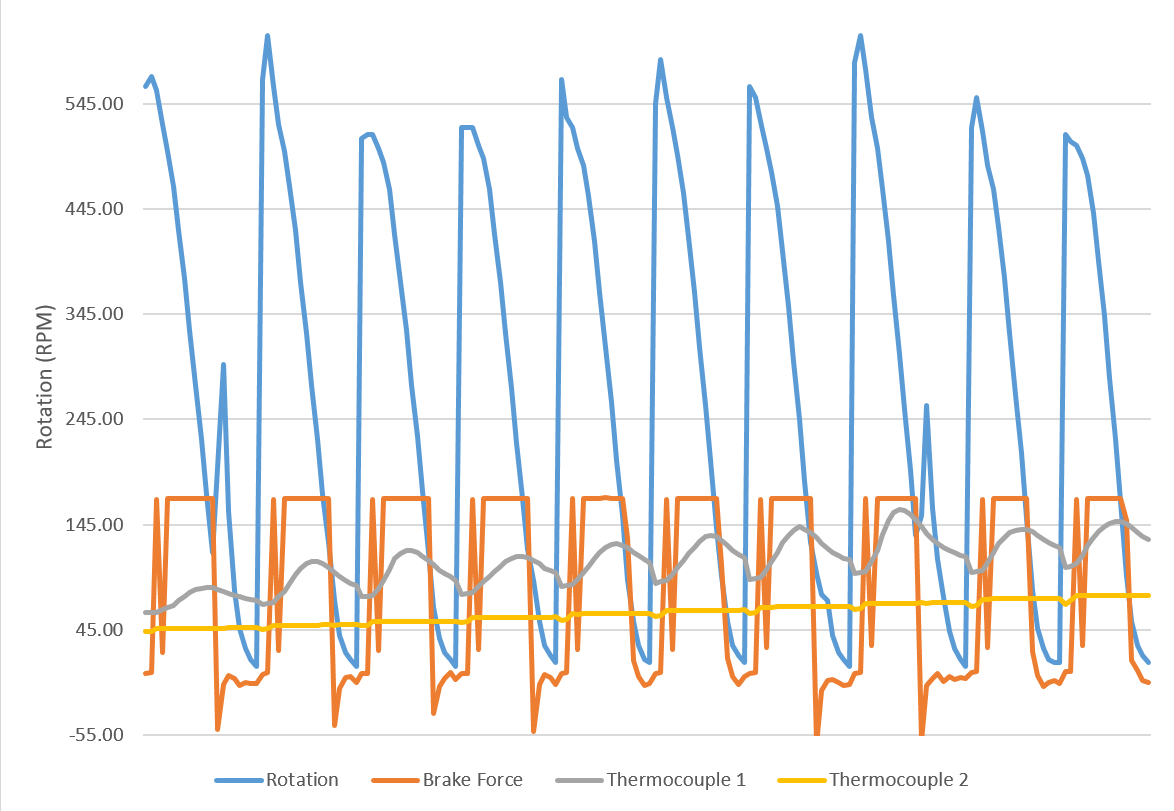
\includegraphics[width=.8\textwidth]{figuras/fig-test-first-ten-snubs}
				\caption{Measurements of the first ten snubs of the test}
				\label{fig:test-first-ten-snubs}
		\end{figure}

		Based on experiment results, it is possible to see the correlation between the measured quantities. Clearly the measured rotation falls rapidly as the brake force saturates to a maximum brake force value. Moreover, at each brake event, detected when the brake force increases, the temperature measured on each of thoose thermocouples increases.
		\par

		Taking a more detailed look at the temperature variation at each snub, Figure \ref{fig:test-first-ten-snubs-force-temperature} show the measured brake force regard the measured temperature at the first ten snubs. This graph states the corelation between the temperature of the brake pads and the braking action, and the fact that the temperature increases during the braking act is perfectly in agreement with the fact that a braking system can be analysed as a kinectic to thermal energy converter, at is was explained in Section \ref{sec:working-principles-of-disk-brake-systems}.

		\begin{figure}[htbp]
				\centering
				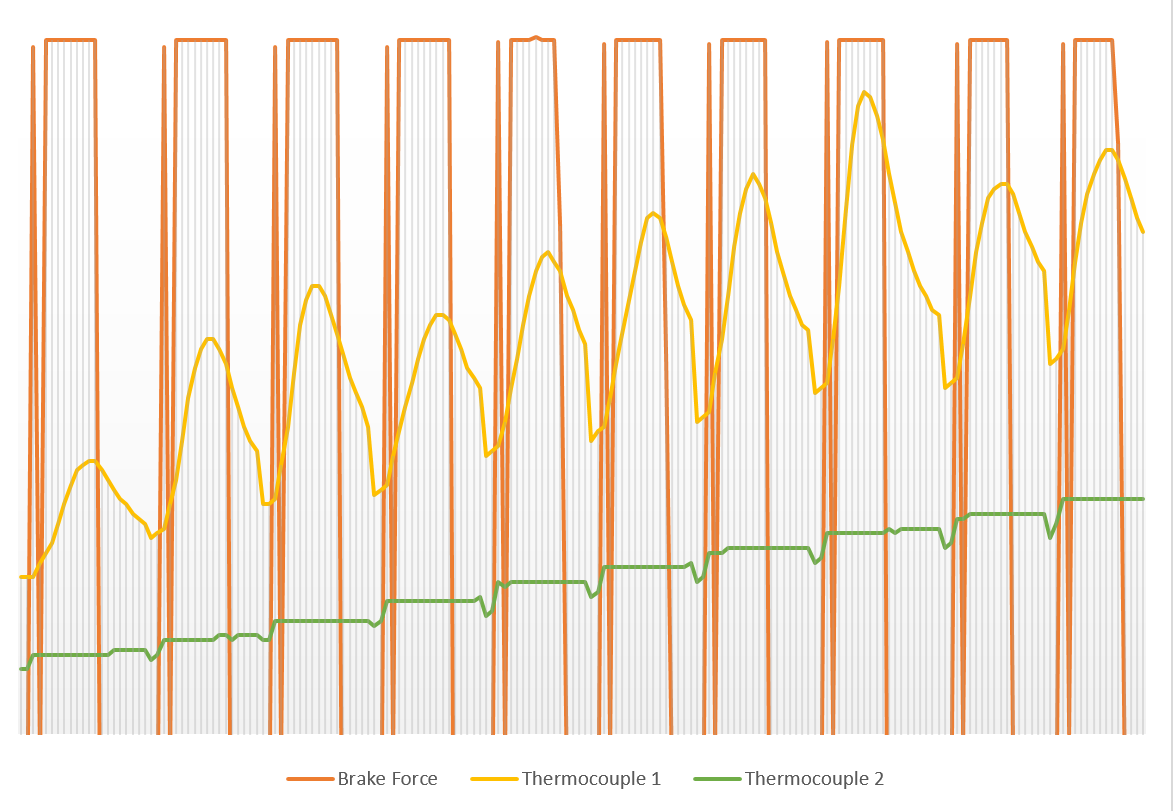
\includegraphics[width=.8\textwidth]{figuras/fig-test-first-ten-snubs-force-temperature}
				\caption{Temperature and Brake Force Measurements of The First Ten Snubs}
				\label{fig:test-first-ten-snubs-force-temperature}
		\end{figure}

		\par

		Whereas the temperature increases at each snub, there may be a point where the temperature reaches a equilibrium, Figure \ref{fig:test-temperature} shows the variation of temperature during the 100 snubs, it is possible to see that even that the temperature bounces at each snub, there may be a point were the temperature stabilizes close to a certain temperature.

		\begin{figure}[htbp]
				\centering
				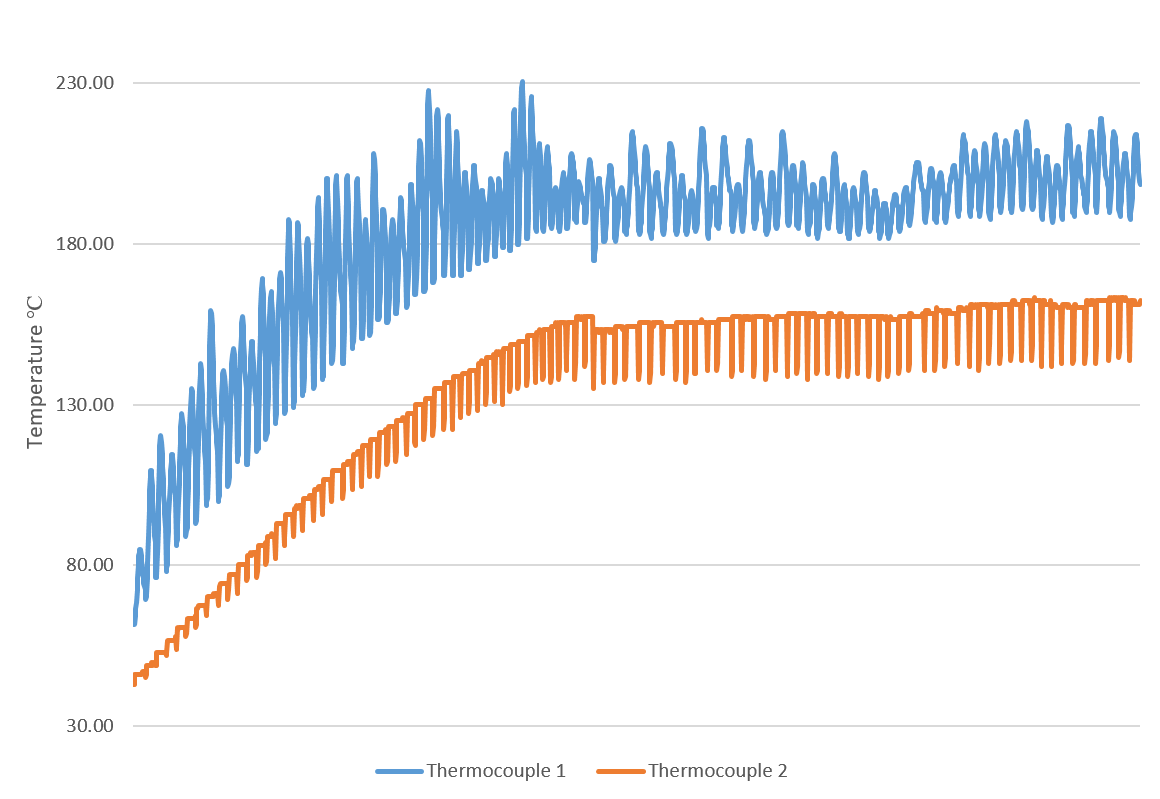
\includegraphics[width=.8\textwidth]{figuras/fig-test-temperature}
				\caption{Temperature Variation During The Whole Test}
				\label{fig:test-temperature}
		\end{figure}
		\par

		Another interesting point to analyse is the effect of the temperature of the pads and the rate of desaceleration of the rotor. Figure \ref{fig:snubs-rotation} shows the desaceleration curves at each snub and shows that during the test the brake efficiency was slightly reduced as the temperature would increase.

		\begin{figure}[htbp]
				\centering
				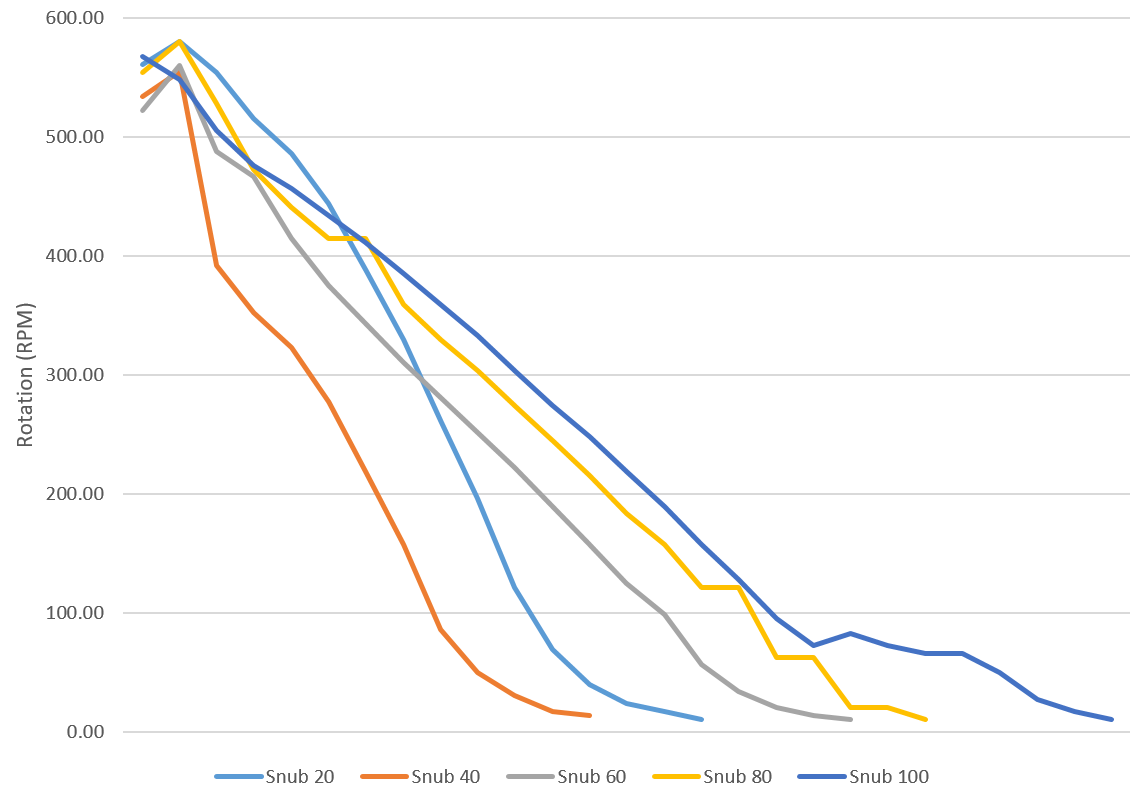
\includegraphics[width=.8\textwidth]{figuras/fig-snubs-rotation}
				\caption{Deceleration During the Whole Test}
				\label{fig:snubs-rotation}
		\end{figure}

\section{Analog Output Tests}\label{sec:analog-output-test}
	
	\subsection{Analog Output Duty Cycle Tests}\label{sec:duty-cycle-test}

		In order to test the analog output of the system an additional test using just a serial terminal was performed to validade the analog output and its usage. Before starting this test the frequency inverter was configured to take the 0-10V analog input as its speed reference with a gain of two and maximum rotation of 500rpm. Whereas, when 5V is present at this analog input the rotor should spin at a rotation close to 500rpm and when 2.5V is present at the input the rotor should spin at a rotation close to 250rpm.
		\par
		The test was carried out varying the analog output from 50 to 100$\%$ duty cycle (2.5 to 5V), taking 50 samples at every 10$\%$ interval, \textit{i.e.} taking 50 samples at 50$\%$, 50 samples at 60$\%$, 50 samples at 70$\%$, 50 samples at 80$\%$, 50 samples at 90$\%$ and finally 50 samples at 100$\%$. At each sample the CKP acquisition channel and the analog output feedback channel were monitored.
	
	\subsection{Results and Discussion}\label{sec:duty-cycle-test-results}
		Figure \ref{fig:test-analog-voltage} shows the analog output voltage in respect with the duty cycle.

		\begin{figure}[htbp]
				\centering
				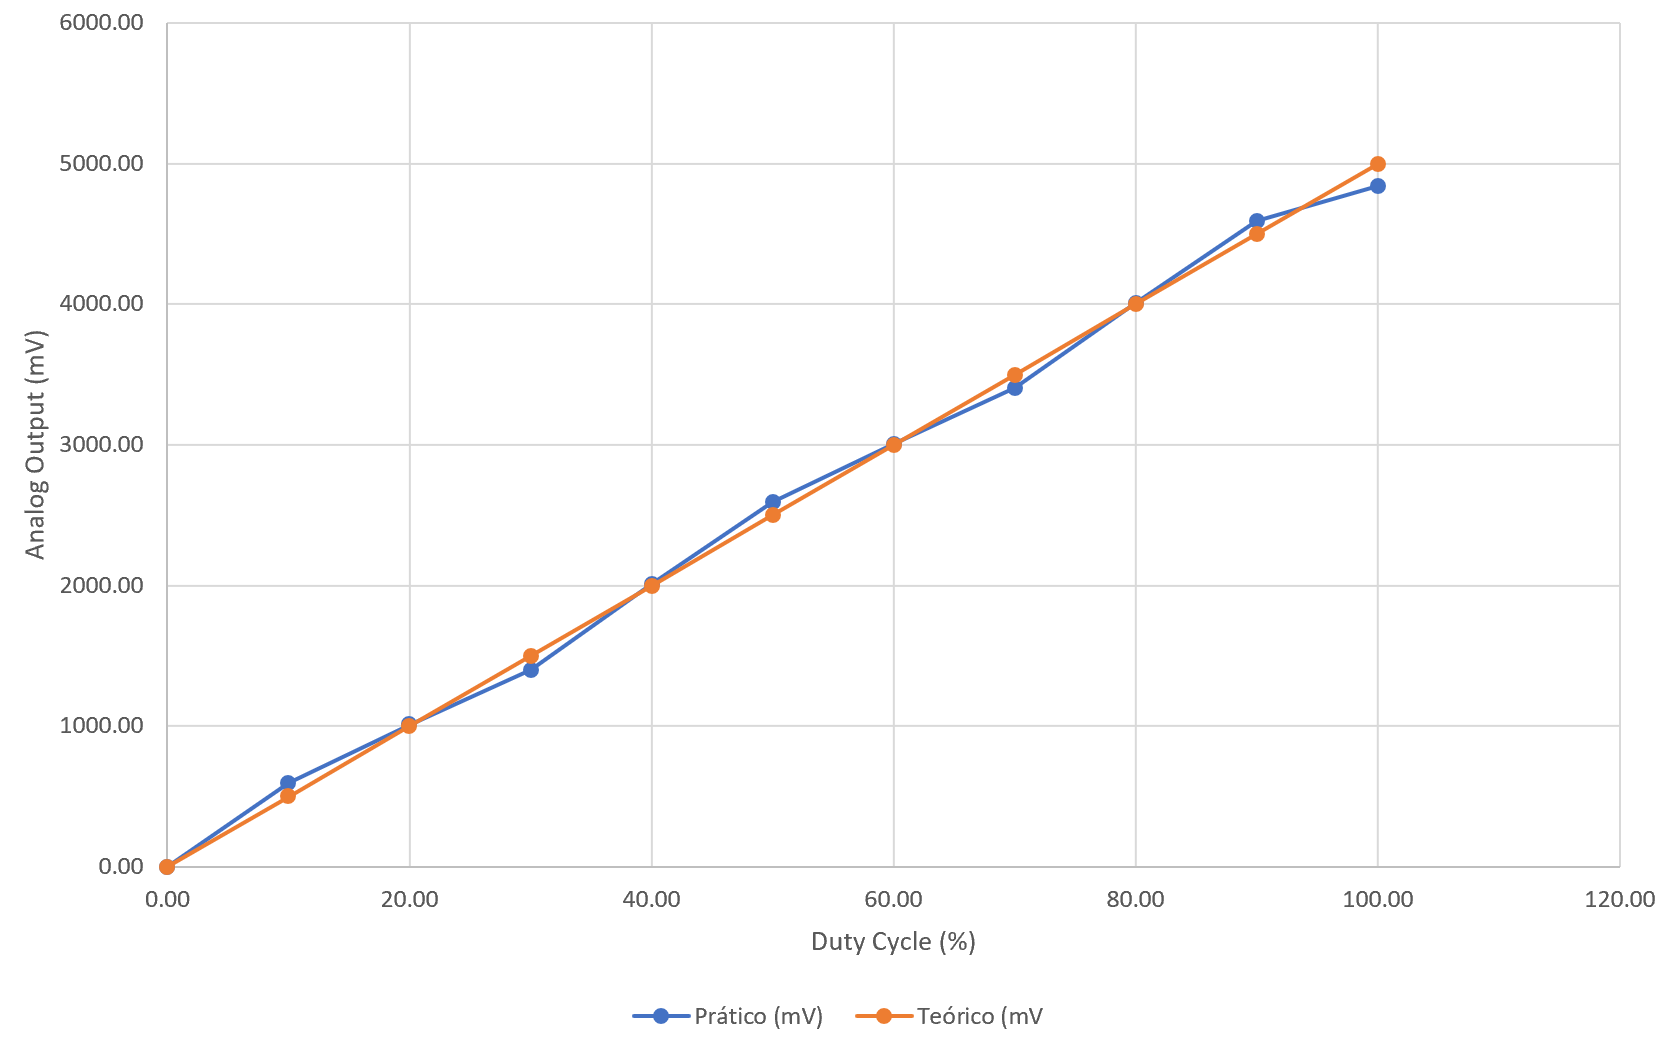
\includegraphics[width=1\textwidth]{figuras/fig-test-analog-voltage}
				\caption{Analog Output in Respect with Duty Cycle}
				\label{fig:test-analog-voltage}
		\end{figure}

		It is possible to see that the measured output was really faithful to the theoretically calculated output, the average error was just 3.35$\%$ which is pretty low. If we disconsider the measured values from 0$\%$ and 100$\%$ this erros falls to 1.58$\%$, probably this is related to the fact that 0$\%$ and 100$\%$ produces a theoretically output of 0V and 5V, which is respectively the negative and positive supply of the operational amplifier from the analog output circuit (check Section \ref{ssec:pwm-to-speed-reference-circuit}). Although the error for 0$\%$ and 100$\%$ is more than two times the error from the rest of the possible duty cycles, it still is quite small, and this happens because the choosen amplifier for the analog output circuit has rail-to-rail input/output.
		\par

		Different from the brake tests from Sections \ref{ssec:full-stop-test} and \ref{ssec:full-stop-test-results}, the frequency inverter was always on, the consequence of this is that the noise from the electric motor and the frequency inverter was always interfering with the CKP sensor signal. Figure \ref{fig:test-analog-rotation} shows the measured rotation in respect with the duty cycle.

		\begin{figure}[htbp]
				\centering
				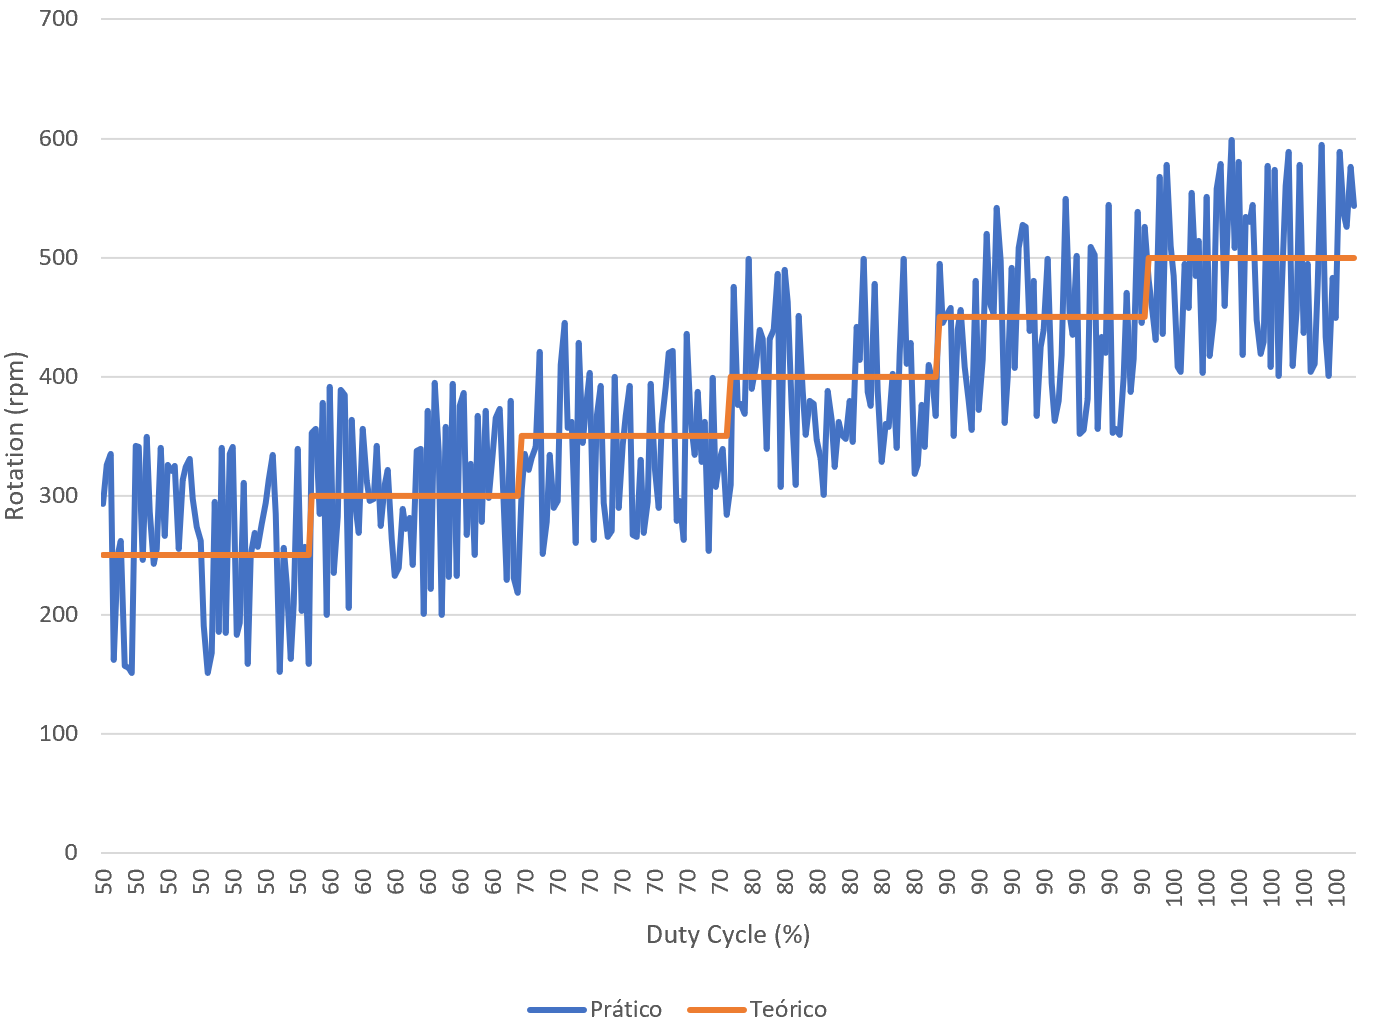
\includegraphics[width=1\textwidth]{figuras/fig-test-analog-rotation}
				\caption{Rotation in Respect with Duty Cycle}
				\label{fig:test-analog-rotation}
		\end{figure}

		The signal is extremely noisy, compared to the theoretical rotation. However, even with all that noise it is possible to see that the signal is varying within a range close to the desired rotation. Maybe with a more sophisticated software it would be possible to treat this signal better to achieve better results.